\section{Introduction} \label{sec:introduction}
\noindent
This document describes the design methodology, implementation, and usage of KitFox.
KitFox is a modeling framework of multi-physics libraries for integrated power, thermal, and reliability simulation of multicore microarchitectures.
The goal of KitFox framework is to facilitate the microarchitectural explorations at the intersection of applications, microarchitectural performance, and various physical phenomena including energy, power, thermal, and lifetime reliability.
KitFox is based on the integration of models that simulate different physical properties, including the popular tools in the architecture community such as HotSpot and McPAT.
Each model in KitFox is encapsulated into a standard class called \emph{library} (e.g., energy, thermal, or reliability library).
Any new or updated models can be seamlessly integrated into KitFox by encapsulating them into the respective library. 
There are no hidden software dependencies between libraries, and all interactions are explicitly managed via the standard library interface that avoids modifications to the third-party tools.
The interface to the multicore simulator is through an application programming interface (API) that relieves the microarchitecture modeler from orchestrating all multi-physics interactions.
Figure \ref{fig:kitfox_concept} illustrates the concept of standard libraries and user API. Towards this goal, KitFox has the following features and contributions.

\begin{itemize}
\item{\emph{Standard Library}: Each model is encapsulated into standard class called \emph{library} and integrated to KitFox. No cross-dependency in software integration is created between the models, and any new models can be added to the framework.} 
\item{\emph{Interacting Library Models}: Interactions between the physical models are orchestrated inside KitFox via the standard library interface. It minimizes user involvement in data management to coordinate multiple libraries and subclass models.} 
\item{\emph{Simple User API}: KitFox provides a set of user API functions to be used in microarchitecture simulations. The same function is used for calculating the same physical property via the standard library interface, regardless of which individual model is used inside the framework.}
\item{\emph{Configurable Processor Model}: KitFox provides a configuration method that users can define the microarchitectural and physical hierarchy of a processor package and associate individual physical models with constituent processor components to be simulated.} 
\item{\emph{Parallel Simulation via MPI Interface}: KitFox supports parallel simulation of physical models via the message passing interface (MPI). A microarchitecture simulator and KitFox can execute in parallel in separate MPI processes, and KitFox itself can also be parallelized into multiple MPI ranks.}
\end{itemize}

\begin{figure}[h]
\centering
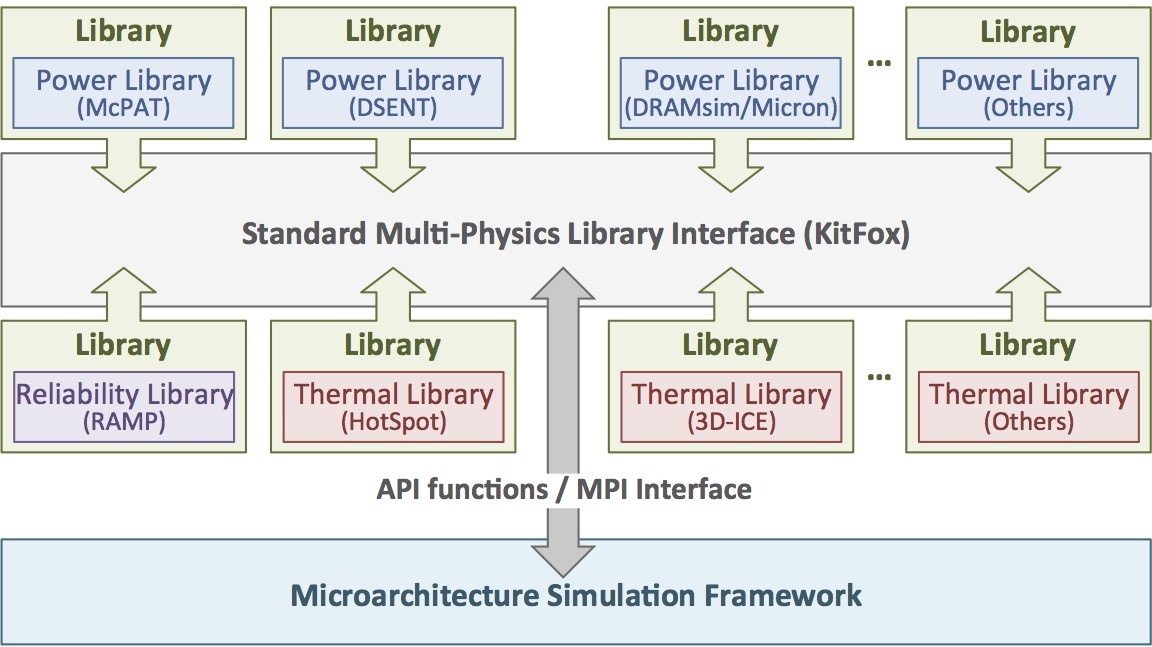
\includegraphics[width=0.6 \textwidth]{figures/kitfox_concept.jpg}
\caption{Multiple physical models are integrated into KitFox as \emph{libraries}. It standardizes the integration and use of models, and provides microarchitecture simulators with a set of API functions.}
\label{fig:kitfox_concept}
\end{figure}

